\chapter{常用命令使用}
\label{sec:BasicCommand}

\section{命令行下的快捷键}
\label{shortcut}

经常在命令行下工作的小伙伴们,可能用的最多的就是两个上下方向键,主要用来调出
历史命令;使用左右箭头使光标向后或向前移动以修改上次使用过的命令。其实
这样做效率并不是很高,有了快捷键可以让我们的效率提高数倍,而且看起来还
更专业、更加Awesome、更加Geek。掌握了这些快捷键,我们可以做到手不离主键
盘区域,完全可以忽略掉键盘上的四个可爱的箭头。当我们熟练之后,会越发喜
欢这种方式。

\subsection{常用快捷键介绍}

下面介绍一些作者在命令行下经常使用的快捷键,这些快捷键在Emacs下面是有同
样的效果的,不信?你可以试试看。其实,Emacs是Gnu/Linux系统下的命令行编
辑器,通过/etc/profile或/etc/bashrc等文件都可以找到相关的设置。

\begin{enumerate}[itemsep=0pt,parsep=0pt]
	\item Ctrl+A\index{Ctrl+A}快捷键
  \begin{quote}
    这里的A可以理解为Head。当我们按下此组合键时,光标就从当前位置移到了
    命令行的起始位置。别只顾着看,动手试试!
  \end{quote}

\item Ctrl+B\index{Ctrl+B}快捷键
  \begin{quote}
    这里的B可以理解为Backward,向后的意思。有时在命令行上,我们把某个命
    令的参数或路径写错了,一般的做法是,使用左箭头,使光标移动到指定的
    位置,然后修改。其实我们完全可以使用Ctrl+B的方式以达到同样的效果。
    别只顾着看,动手试试!
  \end{quote}

\item Ctrl+C\index{Ctrl+C}快捷键
  \begin{quote}
    这个组合键是用来终止当前正在运行的前台进程。在UNIX环境高级编程一书
    上看到了一个用来终止当前运行进程的组合键,是Ctrl+\textbackslash
    \cite{unixenvironment}。别只顾着看,动手试试!
  \end{quote}

\item Ctrl+D\index{Ctrl+D}快捷键
  \begin{quote}
    这个组合键的用途也很广,我主要用此组合键来退出某个程序,如Python、
    MySQL等等。在命令行下意思就不同啦,此时的D可以理解为Delete。按下此
    组合键,会删除当前光标处的字符。别只顾着看,动手试试!
  \end{quote}

\item Ctrl+E\index{Ctrl+E}快捷键
  \begin{quote}
    这里的E可以理解为End。当在命令行按下此组合键时,我们的可爱的光标就
    乖乖地跑到了当前命令行的最后。\marginpar{这是边注一个}
  \end{quote}

\item Ctrl+F\index{Ctrl+F}快捷键
  \begin{quote}
    这里的F可以理解为Forward,向前的意思,等同于按下右箭头。别只顾着看,
    动手试试!
  \end{quote}

\item Ctrl+H\index{Ctrl+H}快捷键
  \begin{quote}
    此组合键相当于键盘上的Backspace键。按下此组合键,它会从当前光标处开
    始向后删除字符。别只顾着看,动手试试!
  \end{quote}

\item Ctrl+J\index{Ctrl+J}快捷键
  \begin{quote}
    此组合键相当于键盘的回车键。按下此组合键,相当于按了一次回车键。在
    Windows的命令行下,Ctrl+M好像是等同于回车键。别只顾看着,动手试试!
  \end{quote}

\item Ctrl+K\index{Ctrl+K}快捷键
  \begin{quote}
    这里的K可以理解为Kill。按下此组合键,会删除从当前光标到本命令行的结
    束的位置的所有字符。别只顾着看,动手试试!
  \end{quote}

\item Ctrl+L\index{Ctrl+L}快捷键
  \begin{quote}
    这里的L可以理解为Clear。按下此组合键相当于执行了clear这条命令,清除
    当前屏幕上的内容。别只顾着看,动手试试!
  \end{quote}

\item Ctrl+N\index{Ctrl+N}快捷键
  \begin{quote}
    这里的N可以理解为Next。这个组合键的作用是用来调出下一条历史命令,与
    之对应的快捷键Ctrl+P是调出上一条历史命令。代替了向下的箭头。别只顾
    着看,动手试试!
  \end{quote}

\item Ctrl+P\index{Ctrl+P}快捷键
  \begin{quote}
    这里的N可以理解为Previous。这个组合键的作用是用来调出上一条历史命令,
    与之对应的快捷键Ctrl+N是调出下一条历史命令。代替了向上的箭头。别只
    顾着看,动手试试!
  \end{quote}

\item Ctrl+R\index{Ctrl+R}快捷键
  \begin{quote}
    这个组合键是用来搜索之前的历史命令。这里的R可以理解为Reverse,反向
    的意思。在Emacs里为向后搜索,与之对应的是Ctrl+S快捷键是向前搜索。不
    过Ctrl+S在命令行里却不是这个作用,而是用来锁屏的。别只顾着看,动手
    试试!
  \end{quote}

\item Ctrl+S\index{Ctrl+S}快捷键
  \begin{quote}
    这个组合键在Emacs里为向后搜索,与之对应的是Ctrl+S快捷键是向前搜索。不
    过Ctrl+S在命令行里却不是这个作用,而是用来锁屏的。别只顾着看,动手
    试试!锁了之后怎么解锁呢?可以是试试Ctrl+Q组合键。
  \end{quote}

\item Ctrl+T\index{Ctrl+T}快捷键
  \begin{quote}
    此组合键是交换两个相邻字符的位置。交换的是当前光标处字符及其当前光
    标前面的字符。比如我们不小心把clear命令写成了clera,此时我们也不用
    把ra两个字符删掉,然后再写上正确的。此时使我们的光标位于字符a上,让
    后按下此组合键,是不是神奇的事情发生了?当然,如果光标在行尾,按下
    此组合键,它会交换光标前的两个连续的字符。在Emacs下面,使用Ctrl+X与
    Ctrl+T两个组合键\footnote{先按下Ctrl+X,然后松开X,继续
      按着Ctrl键,然后再按下T键,即可完成两个组合键的操作。别嫌麻烦,习
      惯就好了。},可以交换当前光标行与上一行的位置。别只顾着看,动手试
    试!
  \end{quote}

\item Ctrl+W\index{Ctrl+W}快捷键
  \begin{quote}
    此组合键在Emacs中的作用是剪切选中区域的文本。在命令行上使用该组合键
    则是往后删除一个字符组合。也就是说,删除光标左边的一个字母组合或单
    词。比如,我们在此命令行上使用了命令如下,“service network
    restart”,让我们的光标位于字符串的restart的后面,按下该组合键,看看
    有何效果?是不是变成“service network”了?确实是这样,如果我们使用
    Backspace键的话,则需要使用7次的按键才能达到一个Ctrl+W的组合键的效
    果。嗯,别只顾着看,动手试试?
  \end{quote}

\item Alt+.\index{Alt+.}快捷键
  \begin{quote}
    此组合键是调出上一条命令的最后一个参数。如上一条命是“service
    network restart”,则“restart”就是最后一个参数。如果我们接下来要敲的
    命令需要用到上一条命令的最后一个参数,则可使用此快捷键,而不需要手
    工输入“restart”了,而且不会出错,节省敲击键盘的次数。如果我们接下来
    想重启httpd服务,则只需要输入“service httpd ”,然后按下“Alt+.”即可
    补全上一条命令的“restart”。在有些终端上,按“Alt+.”组合键可能会没有
    效果,这时可以使用“ESC+.”组合键代替。在Emacs中,ESC键与Alt键是等价
    的。可以动手试试该组合键的效果。
  \end{quote}

\end{enumerate}


\section{使用man page获得帮助}
\label{sec:getHelp}

当我们遇到不会用的系统命令时,该怎么办呢?或许你第一个想到的
是百度或谷歌,这样想很正常,可以节省很多时间。如果每次遇到不会的命令,
都去找网络,个人觉得这不是一件好的事情,不利于我们自身的提高。
在开源界遇到了问题,有一句口号是:“有问题,找男人\footnote{并不是真男人,而是man page}”。

如果不依靠互联网,该怎么解决呢?那就是依赖系统自带的man page\index{man
  page}了。通过它我们可以获取绝大部分的系统帮助信息。



\section{echo与终端颜色}
\label{sec:echoCmd}

echo\index{echo}会将输入的字符串送往标准输出。输出的字符串间以空白字符隔开, 并在最
后加上换行号。

参数:

\begin{enumerate}[itemsep=0pt,parsep=0pt]
\item \-n 不要在最后自动换行 
\item \-e 若字符串中出现以下字符,则特别加以处理,而不会将它当成一般文字输出: 
\begin{verbatim}
\a 发出警告声; 
\b ***前一个字符; 
\c 最后不加上换行符号; 
\f 换行但光标仍旧停留在原来的位置; 
\n 换行且光标移至行首; 
\r 光标移至行首,但不换行; 
\t 插入tab; 
\v 与\f相同; 
\\ 插入\字符; 
\nnn 插入nnn(八进制)所代表的ASCII字符; 
–help 显示帮助 
–version 显示版本信息
\end{verbatim}
\end{enumerate}

\subsection{终端颜色}

echo字体颜色和背景颜色 

-e enable interpretation of the backslash-escaped characters listed below 

字背景颜色范围:40-47

\begin{table}[!htbp]
  \centering
  \begin{tabular}{llll}
    \toprule
    R & G & B & Color \\
    \midrule
    0 & 0 & 0 & Black \\
    0 & 0 & 1 & Blue \\
    0 & 1 & 0 & Green \\
    0 & 1 & 1 & Cyan \\
    1 & 0 & 0 & Red \\
    1 & 0 & 1 & Magenta \\
    1 & 1 & 0 & Yellow \\
    1 & 1 & 1 & White \\
    \bottomrule
  \end{tabular}
  \caption{颜色表\cite{computersystem}}
  \label{tab:colorTable}
\end{table}

\begin{verbatim}
40:黑 
41:深红 
42:绿 
43:*** 
44:蓝色 
45:紫色 
46:深绿 
47:白色
\end{verbatim}

字颜色:30-37

ANSI控制码的说明:

\begin{verbatim}
\e[0m 关闭所有属性 
\e[1m 设置高亮度 
\e[4m 下划线 
\e[5m 闪烁 
\e[7m 反显 
\e[8m 消隐 
\e[30m — \e[37m 设置前景色 
\e[40m — \e[47m 设置背景色 
\e[nA 光标上移n行 
\e[nB 光标下移n行 
\e[nC 光标右移n行 
\e[nD 光标左移n行 
\e[y;xH设置光标位置 
\e[2J 清屏 
\e[K 清除从光标到行尾的内容 
\e[s 保存光标位置 
\e[u 恢复光标位置 
\e[?25l 隐藏光标 
\e[?25h 显示光标
\end{verbatim}

下面看一个例子:
\begin{verbatim}
for i in `seq 0 7` ; do echo -e "\033[30;4${i}m      \033[0m"; \ 
done
\end{verbatim}

输出结果为:
\begin{figure}[hbtp]
  \centering
  
\includegraphics[width=.15\textwidth]{img/color.png}
  \caption{终端颜色效果}
  \label{fig:TermColor}
\end{figure}


\section{date命令的使用}
\label{sec:dateCmd}

\index{date}

\small{
\begin{verbatim}
# 设日期
date -s 20091112                     

# 设时间
date -s 18:30:50                     

# 7天前日期
date -d "7 days ago" +%Y%m%d         

# 5分钟前时间
date -d "5 minute ago" +%H:%M        

# 一个月前
date -d "1 month ago" +%Y%m%d        

# 日期格式转换
date +%Y-%m-%d -d '20110902'         

# 日期和时间
date +%Y-%m-%d_%X                    

# 纳秒
date +%N                             

# 换算成秒计算(1970年至今的秒数)
date -d "2012-08-13 14:00:23" +%s    

# 将时间戳换算成日期
date -d "@1363867952" +%Y-%m-%d-%T   

# 将时间戳换算成日期
date -d "1970-01-01 UTC 1363867952 seconds" +%Y-%m-%d-%T  

# 格式化系统启动时间(多少秒前)
date -d "`awk -F. '{print $1}' /proc/uptime` second ago" +"%Y-%m-%d %H:%M:%S"    
\end{verbatim}
}
\normalsize

\section{yum命令的使用}
\label{sec:yumCmd}
\index{yum}
安装好系统时,在/etc/yum.repos.d目录下回有一个rhel-debuginfo.repo的文件,
我们这里以redhat系统为例进行讲解。不管这个配置文件的名字如何,但文件的
扩展名须为.repo,如redhat.repo也是可以的。我们需要做一些准备工作。

准备系统镜像文件并挂载到本地:

\small{
\begin{verbatim}
[root@iLiuc ~]# ls 
rhel-server-5.5-i386-dvd.iso

[root@iLiuc ~]# mount -o loop rhel-server-5.5-i386-dvd.iso /media
\end{verbatim}
}
\normalsize

复制镜像里的文件到本地目录:

\begin{verbatim}
[root@iLiuc ~]# mkdir /iso
[root@iLiuc ~]# cp -r /media/* /iso
\end{verbatim}

修改这个配置文件:

\begin{verbatim}
[root@iLiuc ~]# cat /etc/yum.repos.d/rhel-debuginfo.repo
[rhel-debuginfo]
name=Red Hat Enterprise Linux $releasever - $basearch - Debug
baseurl=file:///iso/Server
enabled=1
gpgcheck=0
\end{verbatim}

几点说明:

\begin{quote}
    1. [rhel-debuginfo] 中括号里的内容可以随意写 \\
    2. name 这一行可有可无 \\
    3. baseurl 这行要指定我们的资源在哪里 \\
    4. file:// 说明我们使用什么协议,也可以是ftp://等 \\
    5. /iso/Server 指明我们的源在 /iso/Server 目录下
\end{quote}

配置好之后,如何使用呢?直接看操作吧:

\begin{enumerate}[itemsep=0pt,parsep=0pt]
\item 列出我们有哪些yum仓库
  \small{
\begin{verbatim}
[root@iLiuc ~]# yum repolist
\end{verbatim}
  }
  \normalsize

\item 列出仓库里的包
\begin{verbatim}
[root@iLiuc ~]# yum list
Deployment_Guide-en-US.noarch    5.2-11               installed     
GConf2.i386                      2.14.0-9.el5         installed     
ImageMagick.i386                 6.2.8.0-4.el5_1.1    installed     
MAKEDEV.i386                     3.23-1.2             installed     
NetworkManager.i386              1:0.7.0-10.el5       installed     
NetworkManager-glib.i386         1:0.7.0-10.el5       installed     
NetworkManager-gnome.i386        1:0.7.0-10.el5       installed     
ORBit2.i386                      2.14.3-5.el5         installed    
....
yum-utils.noarch                 1.1.16-13.el5        rhel-debuginfo
yum-verify.noarch                1.16-13.el5          rhel-debuginfo
yum-versionlock.noarch           1.1.16-13.el5        rhel-debuginfo
zisofs-tools.i386                1.0.6-3.2.2          rhel-debuginfo
zsh.i386                         4.2.6-3.el5          rhel-debuginfo
zsh-html.i386                    4.2.6-3.el5          rhel-debuginfo
\end{verbatim}
\end{enumerate}

一些说明:
\begin{quote}
    1. 第一列是我们的软件包名 \\
    2. 第二列是对应软件包的版本号 \\
    3. 第三列 \\
    + installed表明该软件包已安装 \\
    + rhel-debuginfo表明包未安装 
\end{quote}

几个常用的yum命令:
\begin{table}[!htbp]
  \centering
    \caption{yum常用命令选项}
    \begin{tabular}{ll}
      \toprule
      命令           & 说明 \\
      \midrule
      repolist       & 列出我们有哪些yum仓库 \\
      list           & 列出仓库里有哪些软件包 \\
      install        & 安装软件包的命令 \\
      groupinstall   & 安装软件包组 \\
      erase          & 移除一个或多个软件包 \\
      whatprovides   & 查询一个命令属于哪个安装包 \\
      \bottomrule
    \end{tabular}
\end{table}

\subsection{一些实例}
\label{sec:yumExamples}

% \section{zypper命令的使用}
\label{sec:zypperCmd}

\subsection{zypper本地源的配置}
\label{subsec:zypperLocalrepo}

SUSE的zypper本地源配置起来跟yum的配置很相似,它们的配置文件有很多相似之
处。不过,个人觉得zypper这个工具稍微强大些。在SUSE下,可以通过一条
zypper的命令,即可完成zypper源的配置。

为什么会有本节内容呢?主要是2014年9月26日,Bash爆出了一个漏洞,传闻比
“心脏出血”漏洞还要猛,不知道是不是真的。以下是网上给出的验证方法,测试
环境在我的RHEL6 64bit的虚拟机上,

\small{
\begin{verbatim}
[root@master ~]# env x='() { :;}; echo vulnerable' bash -c "echo this is a test"
vulnerable
this is a test
\end{verbatim}
}
\normalsize

同样,在我的SUSE 11sp2 64bit上运行也是同样的输出,输出内容略。以下几个
包是SUSE的OEM厂商给出的Bash最新的升级包。

\begin{verbatim}
funny:~ # unzip CVE-2014-6271.zip 
Archive:  CVE-2014-6271.zip
   creating: CVE-2014-6271/
  inflating: CVE-2014-6271/bash 9740.htm  
  inflating: CVE-2014-6271/bash-3.2-147.20.1.x86_64.rpm  
  inflating: CVE-2014-6271/bash-doc-3.2-147.20.1.x86_64.rpm  
  inflating: CVE-2014-6271/libreadline5-32bit-5.2-147.20.1.x86_64.rpm  
  inflating: CVE-2014-6271/libreadline5-5.2-147.20.1.x86_64.rpm  
  inflating: CVE-2014-6271/license_agreement.txt  
  inflating: CVE-2014-6271/readline-doc-5.2-147.20.1.x86_64.rpm
\end{verbatim}

接下来的操作是把这些包放到一个目录里,然后把该目录做成系统的一个更新源。
比如,把解压后的目录放到/opt目录下,然后使用zypper ar添加该zypper源。

\small{
\begin{verbatim}
funny:~ # mv CVE-2014-6271 /opt/update
funny:~ # zypper ar file:///opt/update update
Adding repository 'update' [done]
Repository 'update' successfully added
Enabled: Yes
Autorefresh: No
GPG check: Yes
URI: file:/opt/update
\end{verbatim}
}
\normalsize

接下来,使用zypper lr验证下,

\small{
\begin{verbatim}
funny:~ # zypper lr
# | Alias  | Name   | Enabled | Refresh
--+--------+--------+---------+--------
1 | local  | local  | Yes     | Yes    
2 | update | update | Yes     | No
\end{verbatim}
}
\normalsize

说明我们已成功添加update的源。另外,执行”zypper ar URI alias“后,会在
/etc/zypp/repo.d/目录下生成alias.repo配置文件。接下来,我们试试zypper
update命令,看是不是可以真的可以升级?

\small{
\begin{verbatim}
funny:~ # zypper update
Building repository 'update' cache [done]
Loading repository data...
Reading installed packages...

The following packages are going to be upgraded:
  bash bash-doc libreadline5 readline-doc 

The following packages are not supported by their vendor:
  bash bash-doc libreadline5 readline-doc 

4 packages to upgrade.
Overall download size: 923.0 KiB. ...
Continue? [y/n/?] (y): y
Retrieving package libreadline5-5.2-147.20.1.x86_64 (1/4), ...
Retrieving package bash-3.2-147.20.1.x86_64 (2/4), ...
Retrieving package readline-doc-5.2-147.20.1.x86_64 (3/4), ...
Retrieving package bash-doc-3.2-147.20.1.x86_64 (4/4), ...
Retrieving package libreadline5-5.2-147.20.1.x86_64 (1/4), ...
Installing: libreadline5-5.2-147.20.1 [done]
Retrieving package bash-3.2-147.20.1.x86_64 (2/4), ...
Installing: bash-3.2-147.20.1 [done]
Retrieving package readline-doc-5.2-147.20.1.x86_64 (3/4), ...
Installing: readline-doc-5.2-147.20.1 [done]
Retrieving package bash-doc-3.2-147.20.1.x86_64 (4/4), ...
Installing: bash-doc-3.2-147.20.1 [done]
\end{verbatim}
}
\normalsize

以上说明可以进行升级的。接下来,我们使用zypper ps命令,可以查看有哪些终
端还在使用之前没有升级过的bash,

\small{
\begin{verbatim}
funny:/etc/zypp/repos.d # zypper ps
The following running processes use deleted files:

PID   | PPID  | UID | Login | Command | Files                    
------+-------+-----+-------+---------+--------------------------
2663  | 2542  | 0   | root  | bash    | /lib64/libreadline.so.5.2
      |       |     |       |         | /bin/bash (deleted)      
22426 | 22423 | 0   | root  | bash    | /lib64/libreadline.so.5.2
      |       |     |       |         | /bin/bash (deleted)      

You may wish to restart these processes.
\end{verbatim}
}
\normalsize

说明还有bash升级前的两个进程还在运行,我们可以退出这两个终端,再次登入
系统,再次使用zypper ps命令来查看,就会看到”No processes using deleted
files found.“的提示。

\subsection{zypper命令选项介绍}
\label{subsec:zypperCmdopt}

zypper\index{zypper}是SuSE\index{SUSE}系列下面的包管理工具,如同
\ref{sec:yumCmd}节的yum工具。

zypper的几个重要选项:

\begin{table}[!htbp]
  \centering
    \caption{zypper安装源操作选项}
    \begin{tabular}{ll}
      \toprule
      选项           & 说明 \\
      \midrule
      repos, lr      & 列出库 \\
      addrepo, ar    & 添加库 \\
      renamerepo, nr & 重命名指定的安装源 \\
      modifyrepo, mr & 修改指定的安装源 \\
      refresh, ref   & 刷新所有安装源 \\
      clean          & 清除本地缓存 \\
      \bottomrule
    \end{tabular}
\end{table}

举例说明,

列出当前有哪些库,

\begin{verbatim}
# zypper lr
# | Alias       | Name        | Enabled | Refresh
--+-------------+-------------+---------+--------
1 | 6271        | 6271        | Yes     | No     
2 | 7169        | 7169        | Yes     | No     
3 | SUSE11SP2   | SUSE11SP2   | Yes     | No     
4 | cve20150235 | cve20150235 | Yes     | No
\end{verbatim}

添加本地库,

\begin{verbatim}
# zypper ar file:///opt/patch/ mypatch
Adding repository 'mypatch' [done]
Repository 'mypatch' successfully added
Enabled: Yes
Autorefresh: No
GPG check: Yes
URI: file:/opt/patch/

# zypper lr
# | Alias       | Name        | Enabled | Refresh
--+-------------+-------------+---------+--------
1 | 6271        | 6271        | Yes     | No     
2 | 7169        | 7169        | Yes     | No     
3 | SUSE11SP2   | SUSE11SP2   | Yes     | No     
4 | cve20150235 | cve20150235 | Yes     | No
5 | mypatch     | mypatch     | Yes     | No
\end{verbatim}

zypper的查询选项:

\begin{table}[!htbp]
  \centering
    \caption{zypper工具查选选项}
    \begin{tabular}{ll}
      \toprule
      选项              & 说明 \\
      \midrule
      search, se        & 安装软件包 \\
      info, if          & 查看软件包信息 \\
      packages, pa      & 列出所有可用的软件包 \\
      patterns, pt      & 列出所有可用的模式 \\
      products, pd      & 列出所有可用的产品 \\
      what-provides, wp & 列出能够提供指定功能的软件包 \\
      \bottomrule
    \end{tabular}
\end{table}

举例说明,

\begin{verbatim}
# zypper se snmp
Building repository 'mypatch' cache [done]
Loading repository data...
Reading installed packages...

S | Name                | Summary                         | Type      
--+---------------------+---------------------------------+-----------
i | libsnmp15           | Shared Libraries from net-snmp  | package   
  | libsnmp15-32bit     | Shared Libraries from net-snmp  | package   
i | net-snmp            | SNMP Daemon                     | package   
  | net-snmp            | SNMP Daemon                     | srcpackage
  | perl-Net-SNMP       | Net::SNMP Perl Module           | package   
  | perl-Net-SNMP       | Net::SNMP Perl Module           | srcpackage
i | perl-SNMP           | Perl-SNMP                       | package   
  | php5-snmp           | PHP5 Extension Module           | package   
  | php53-snmp          | PHP5 Extension Module           | package   
  | rsyslog-module-snmp | SNMP support module for rsyslog | package   
i | snmp-mibs           | MIB files from net-snmp         | package
#
# zypper if net-snmp
Loading repository data...
Reading installed packages...


Information for package net-snmp:

Repository: SUSE-Linux-Enterprise-Server-11-SP2 11.2.2-1.234
Name: net-snmp
Version: 5.4.2.1-8.12.6.1
Arch: x86_64
Vendor: SUSE LINUX Products GmbH, Nuernberg, Germany
Support Level: Level 3
Installed: Yes
Status: up-to-date
Installed Size: 1.0 MiB
Summary: SNMP Daemon
Description: 
This package was originally based on the CMU 2.1.2.1 snmp verbatim.It has been greatly modified, restructured, enhanced, and fixed.It hardly looks the same as anything that CMU has ever released.It was renamed from cmu-snmp to ucd-snmp in 1995 and later renamedfrom ucd-snmp to net-snmp in November 2000.
#
\end{verbatim}

zypper软件管理:

\begin{table}[!htbp]
  \centering
    \caption{zypper软件管理选项}
    \begin{tabular}{ll}
      \toprule
      选项               & 说明 \\
      \midrule
      install, in        & 安装软件包 \\
      remove, rm         & 删除软件包 \\
      verify, ve         & 检验软件包依赖关系的完整性 \\
      update, up         & 更新已安装的软件包到新的版本 \\
      dist-upgrade, dup  & 整个系统的升级 \\
      source-install, si & 安装源代码软件包和它们的编译依赖 \\
      \bottomrule
    \end{tabular}
\end{table}

举例说明,

\begin{verbatim}
# zypper rm net-snmp
Loading repository data...
Reading installed packages...
Resolving package dependencies...

The following packages are going to be REMOVED:
  net-snmp perl-SNMP 

2 packages to remove.
After the operation, 1.6 MiB will be freed.
Continue? [y/n/?] (y): y
Removing perl-SNMP-5.4.2.1-8.12.6.1 [done]
Removing net-snmp-5.4.2.1-8.12.6.1 [done]
#
# zypper in -y net-snmp
Loading repository data...
Reading installed packages...
Resolving package dependencies...

The following NEW packages are going to be installed:
  net-snmp perl-SNMP 

2 new packages to install.
Overall download size: 543.0 KiB. After the operation, additional 1.6 MiB will be used.
Continue? [y/n/?] (y): y
Retrieving package perl-SNMP-5.4.2.1-8.12.6.1.x86_64 (1/2), 176.0 KiB (609.0 KiB unpacked)
Retrieving package net-snmp-5.4.2.1-8.12.6.1.x86_64 (2/2), 367.0 KiB (1.0 MiB unpacked)
Installing: perl-SNMP-5.4.2.1-8.12.6.1 [done]
Installing: net-snmp-5.4.2.1-8.12.6.1 [done]
Additional rpm output:
Updating etc/sysconfig/net-snmp...
\end{verbatim}



\section{parted命令的使用}
\label{sec:PartedCmd}

Gnu/Linux系统的分区工具通常可以使用fdisk与parted。我们用的比较多的工具
就是fdisk了,这里不介绍它的使用了。这里简单的介绍如何使用parted工具,对
于分区表通常有MBR分区表和GPT分区表对于磁盘大小小于2T的磁盘,我们可以使
用fdisk和parted命令工具进行分区对于MBR分区表的特点(通常使用fdisk命令进
行分区)所支持的最大磁盘大小:2T最多支持4个主分区或者是3个主分区加上一
个扩展分区对于GPT分区表的特点(使用parted命令进行分区)支持最大
卷:18EB(1EB=1024TB)最多支持128个分区。

对于parted命令工具分区的介绍

最后,fdisk与parted有些差异。fdisk分区完毕后,需要使用“w”命令才能保存
之前所做的一些操作;而parted则是实时的,每一步操作不需要保存,即时生
效。


\section{mount命令的使用}
\label{sec:mountCmd}

如何挂载iso镜像文件呢?我们可以使用一下mount\index{mount}命令:

\small{
\begin{verbatim}
[root@iLiuc ~]# mount -o loop rhel-server-5.5-i386-dvd.iso /mnt
# 意思是把当前目录下的rhel-server-5.5-i386-dvd.iso挂载到/mnt目录下
\end{verbatim}
}
\normalsize


\section{grep命令的使用}
\label{sec:grepCmd}

grep\index{grep}(global regular expression pattern的缩写)。其实可以把它
理解为过滤关键字用的一个程序。具体怎么用,还是看一个实例吧,然后结束本
节内容。

\subsection{常用选项}

\begin{table}[!htbp]
  \centering
  \caption{grep常用选项}
  \begin{tabular}{l|l}
    \hline
    -A NUM  & 打印出紧随匹配的行之后的下文NUM行 \\
    \hline
    -B NUM  & 打印出匹配的行之前的上文NUM行 \\
    \hline
    -C NUM  & 打印出匹配的行的上下文前后各NUM行 \\
    \hline
    -b      & 在输出的每行前面同时打印出当前行在输入文件中的字节偏移量 \\
    \hline
    -c      & 显示匹配的行数 \\
    \hline
    -f file & 从文件file中获取模式,每行一个 \\
    \hline
    -H      & 为每个匹配的文件打印文件名 \\
    \hline
    -I      & 不搜索二进制文件 \\
    \hline
    -i      & 忽略大小写 \\
    \hline
    -l      & 只显示有匹配的文件的文件名 \\
    \hline
    -L      & 只显示未匹配的文件的文件名 \\
    \hline
    -n      & 输出行号 \\
    \hline
    -o      & 只显示匹配字段 \\
    \hline
    -q      & quiet静默模式 \\
    \hline
    -v      & 只显示不匹配的行 \\
    \hline
  \end{tabular}
\end{table}

\subsection{一些实例}

去掉文件里的注释行和空白行
\begin{verbatim}
# cat filename | grep -v ^$ | grep -v ^# | sudo tee squid.conf
\end{verbatim}

这里我们使用grep命令及cut命令一起把eth0上的IP给取出来,看操作:

\begin{verbatim}
  [root@iLiuc ~]# ifconfig eth0
  eth0 Link encap:Ethernet  HWaddr 5A:B6:4E:85:55:44  
  inet addr:192.168.18.18  Bcast:192.168.18.255  Mask:255.255.255.0
  inet6 addr: fe80::58b6:4eff:fe85:5544/64 Scope:Link
  UP BROADCAST RUNNING MULuTICAST  MTU:1500  Metric:1
  RX packets:11655331 errors:0 dropped:0 overruns:0 frame:0
  TX packets:1074797 errors:0 dropped:0 overruns:0 carrier:0
  collisions:0 txqueuelen:1000 
  RX bytes:4001012028 (3.7 GiB)  TX bytes:628740073 (599.6 MiB)
  Interrupt:185

  # 使用grep命令,匹配关键字,缩小范围
  [root@iLiuc ~]# ifconfig eth0 |grep "inet addr"
  inet addr:192.168.18.18  Bcast:192.168.18.255  Mask:255.255.255.0

  # 使用cut命令,把范围再次缩小些
  [root@iLiuc ~]# ifconfig eth0 |grep "inet addr" | cut -d: -f2
  192.168.18.18  Bcast

  # 是不是快出来了,再使用cut一次,IP地址就出来了
  [root@iLiuc ~]# 自己写出来吧,我已经写得很多了!
\end{verbatim}


\section{crontab命令的使用}
\label{sec:crontabCmd}

假想这样一个场景:每天的凌晨两点,领导都会要求你你重启服务器(当然,这
有点变态)。这时,你该怎么办?你是不是每天凌晨两点都要从温暖的被窝里爬
出来,然后远程连接服务器,然后重启服务器,然后重新钻进被窝,然后失眠
了...。每天都如此,我想你一定会奔溃的。

crontab\index{crontab}命令可以解救你!crontab几个字段的说明:

\small{
\begin{verbatim}
  field          allowed values
  -----          --------------
  minute         0-59
  hour           0-23
  day of month   1-31
  month          1-12 (or names, see below)
  day of week    0-7 (0 or 7 is Sun, or use names)
\end{verbatim}
}
\normalsize

\small{
\begin{verbatim}
  # 查看当前用户的crontab
  [root@iLiuc ~]# crontab -l
  */2 * * * * /usr/lib/clear-server/cleargard/cleargard.sh
  上面语句的意思是,每2分钟去执行/usr/lib/clear-server/cleargard目录下的
  cleargard.sh脚本,只要系统一直运行,它就会循环往复的执行。

  # 编辑crontab
  [root@iLiuc ~]# crontab -e
\end{verbatim}
}
\normalsize


\section{find命令的使用}

find\index{find}命令很强大,强大到可以写很多东西。这里就介绍如何简单的
使用。直接看例子吧:

\small{
\begin{verbatim}
# linux文件无创建时间
# Access 使用时间  
# Modify 内容修改时间  
# Change 状态改变时间(权限、属主)
# 时间默认以24小时为单位,当前时间到向前24小时为0天,向前48-72小时为2天
# -and 且 匹配两个条件 参数可以确定时间范围 -mtime +2 -and -mtime -4
# -or 或 匹配任意一个条件

# 按文件名查找
find /etc -name http        

# 查找某一类型文件
find . -type f               

# 按照文件权限查找
find / -perm                 

# 按照文件属主查找
find / -user                 

# 按照文件所属的组来查找文件
find / -group                

# 文件使用时间在N天以内
find / -atime -n             

# 文件使用时间在N天以前
find / -atime +n             

# 文件内容改变时间在N天以内
find / -mtime -n             

# 文件内容改变时间在N天以前
find / -mtime +n             

# 文件状态改变时间在N天前
find / -ctime +n             

# 文件状态改变时间在N天内
find / -ctime -n             

# 查找文件长度大于1M字节的文件
find / -size +1000000c -print 

# 按名字查找文件传递给-exec后命令
find /etc -name "passwd*" -exec grep "root" {} \; 

# 查找文件名,不取路径
find . -name 't*' -exec basename {} \;  

# 批量改名(查找err替换为ERR {}文件
find . -type f -name "err*" -exec  rename err ERR {} \; 

# 查找任意一个关键字
find 路径 -name *name1* -or -name *name2* 
\end{verbatim}
}
\normalsize




\section{top命令的使用}
\label{sec:topCmd}

top\index{top}命令可动态显示服务器的进程信息,用户可以通过按键来刷新当
前状态。别的不多说,给个例子看看:

\begin{verbatim}
Tasks: 202 total,   2 running, 199 sleeping,   0 stopped,   1 zombie
Cpu(s):  7.9%us,  1.9%sy,  0.0%ni, 89.5%id,  0.7%wa,  0.0%hi,  0.0%si,  0.0%st
Mem:   6003152k total,  1909420k used,  4093732k free,    73688k buffers
Swap:  6180860k total,        0k used,  6180860k free,   893544k cached

  PID USER      PR  NI  VIRT  RES  SHR S %CPU %MEM    TIME+  COMMAND                                                   
 3852 richard   20   0 1329m 127m  31m S   22  2.2   2:11.41 vlc                                                                 
 2891 richard    9 -11  418m 6988 4660 S    6  0.1   0:37.86 pulseaudio 
 2880 richard   20   0 1669m  90m  35m S    5  1.6   1:35.32 gnome-shell
 2452 root      20   0  303m  74m  61m S    4  1.3   1:23.90 Xorg
 3051 richard   20   0  872m 200m  52m S    1  3.4   1:32.25 firefox
   10 root      20   0     0    0    0 S    0  0.0   0:00.57 rcuos/2
   77 root      20   0     0    0    0 R    0  0.0   0:01.30 kworker/3:1
  909 root     -51   0     0    0    0 S    0  0.0   0:10.11 irq/48-iwlwifi
 3025 richard   20   0  581m  19m  11m S    0  0.3   0:01.72 gnome-terminal
 3942 richard   20   0 99.6m  15m 5028 S    0  0.3   0:02.35 python
 4025 richard   20   0 17460 1408  980 R    0  0.0   0:00.04 top
    1 root      20   0 24740 2620 1352 S    0  0.0   0:00.88 init
    2 root      20   0     0    0    0 S    0  0.0   0:00.00 kthreadd
    3 root      20   0     0    0    0 S    0  0.0   0:00.08 ksoftirqd/0
    5 root       0 -20     0    0    0 S    0  0.0   0:00.00 kworker/0:0H                                                                            
    6 root      20   0     0    0    0 S    0  0.0   0:01.68 kworker/u16:0
    7 root      20   0     0    0    0 S    0  0.0   0:01.60 rcu_sched
    8 root      20   0     0    0    0 S    0  0.0   0:01.24 rcuos/0
    9 root      20   0     0    0    0 S    0  0.0   0:00.45 rcuos/1
   11 root      20   0     0    0    0 S    0  0.0   0:00.28 rcuos/3
   12 root      20   0     0    0    0 S    0  0.0   0:00.00 rcuos/4
   13 root      20   0     0    0    0 S    0  0.0   0:00.00 rcuos/5
   14 root      20   0     0    0    0 S    0  0.0   0:00.00 rcuos/6
   15 root      20   0     0    0    0 S    0  0.0   0:00.00 rcuos/7
   16 root      20   0     0    0    0 S    0  0.0   0:00.00 rcu_bh
\end{verbatim}

\section{free命令的使用}
\label{sec:freeCmd}

\subsection{常用选项}
\label{subsec:freeOptions}

free 命令是查看系统内存的使用情况的。下面介绍几个常用的选项,

\begin{table}[htbp]
  \centering
    \caption{free常用选项}
    \label{tab:freeSomeOpts}
    \begin{tabular}{cl}
      \toprule
      选项     & 说明 \\
      \midrule
      -m        & 以 MB 为单位显示当前系统的内存使用情况 \\
      -g        & 以 GB 为单位显示当前系统的内存使用情况 \\
      \bottomrule
    \end{tabular}
\end{table}

\subsection{一些实例}
\label{subsec:freeInstances}



\section{xargs命令的使用}
\label{sec:xargsCmd}
\index{xargs}

\section{tr命令的使用}
\label{sec:trCmd}
\index{tr}

\section{tar命令的使用}
\label{sec:tarCmd}

tar\index{tar}命令是一个打包与解包的一个工具,功能很强大。下面介绍一些常用选项及使
用示例。

通用选项:

\begin{table}[htbp]
  \centering
    \caption{tar通用选项}
    \label{tab:tarGeneralOpt}
    \begin{tabular}{cl}
      \toprule
      选项     & 说明 \\
      \midrule
      j        & 使用bzip2的压缩方式 \\
      t        & 列出压缩包里有哪些文件,并不解压 \\
      z        & 使用gzip的压缩方式 \\
      f        & 指定输出的结果文件。该选项是必选的,不管是压缩还是解压缩 \\
      p        & 保留文件的所有权限 \\
      v        & 压缩或解压缩时,查看其打包过程 \\
      \bottomrule
    \end{tabular}
\end{table}

压缩时用的选项:

\begin{table}[!htbp]
  \centering
    \caption{tar压缩选项}
    \label{tab:tarCompressOpt}
    \begin{tabular}{cl}
      \toprule
      选项     & 说明 \\
      \midrule
      c        & 打包时用的选项,选项c与x不能同时出现 \\
      \bottomrule
    \end{tabular}
\end{table}

解压缩用的选项:

\begin{table}[htbp]
  \centering
    \caption{tar解压缩选项}
    \label{tab:tarUncompressOpt}
    \begin{tabular}{cl}
      \toprule
      选项     & 说明 \\
      \midrule
      x        & 解包时用的选项,选项c与x不能同时出现 \\
      \bottomrule
    \end{tabular}
\end{table}

举例说明:

\small{
\begin{verbatim}
  [root@iLiuc ~]# ls
  360fy        CLEAR-VOD-INSTALLPACKGE.V.2.0.8.tar
  这里有两个文件,第一个为目录,第二个为压缩包

  1. 创建tar包,不压缩
  [root@iLiuc ~]# tar -cvf 360fy.tar 360fy
  360fy/
  360fy/clearVodMS_360fy.tar.gz
  360fy/vod_yuezizhongxin.tar.gz
  360fy/clear_360fy.sql
  上面的例子我们使用-v选项,使我们可以看到过程。其中360fy.tar是我们创建的tar包,是针对
  360fy这个目录的,后面可以是一个或多个文件。

  2. 创建tar包,以gzip方式压缩
  [root@iLiuc ~]# tar -czvf 360fy.tar.gz 360fy

  3. 创建tar包,以bzip2的方式压缩
  [root@iLiuc ~]# tar -cjvf 360fy.tar.bz2 360fy

  4. 查看压缩包的内容,并不解压缩
  [root@iLiuc ~]# tar -tf 360fy.tar
  360fy/
  360fy/clearVodMS_360fy.tar.gz
  360fy/vod_yuezizhongxin.tar.gz
  360fy/clear_360fy.sql

  5. 解压缩
  不管是tar包,还是以gzip或bz2压缩的方式,我们使用一下这条命令都是通用的
  [root@iLiuc ~]# tar -xf 360fy.tar
  [root@iLiuc ~]# tar -xf 360fy.tar.gz
  [root@iLiuc ~]# tar -xf 360fy.tar.bz2
  这里我们没有加-v选项,可以加上-v选项以看到解压过程
\end{verbatim}
}
\normalsize


\section{read命令的使用}
\label{sec:readCmd}
\index{read}

\subsection{常用选项}

\subsection{一些实例}

\section{cut命令的使用}
\label{sec:cutCmd}

cut\index{cut}命令有的时候很有用,比如要获得指定的以某个分隔符分割的列
时,它就可以做到。其实还有比它更强大的工具,如sed及awk等,这里并不介绍
它们,后续章节有介绍。这里就不提及了,跳过它们吧。下面直接看例子吧:

\subsection{常用选项}
\label{subsec:cutOptions}

下面介绍几个常用的cut命令的选项,

\begin{table}[htbp]
  \centering
    \caption{cut常用选项}
    \label{tab:cutSomeOpts}
    \begin{tabular}{cl}
      \toprule
      选项     & 说明 \\
      \midrule
      -c        & 按照字符进行分割 \\
      -d        & 指定分割字段的分隔符,默认是tab \\
      -f        & 指定要显示的列 \\
      \bottomrule
    \end{tabular}
\end{table}

\subsection{一些实例}
\label{subsec:cutInstances}

接下来演示cut命令的一些常用示例,比如我们要查看/etc/passwd文件中用户名,由于用户名是位于/etc/passwd文件中的每一行的第一个以冒号为分割的字段,因此,可以使用cut命令轻松实现取出用户名的需求,

\begin{verbatim}
# cut -d: -f1 /etc/passwd

-d 指定区分列的定界,默认是tab
-f 指定要显示的列
-c 按字符来切割,如
# cut -c1-6 file (取文件第一行的前6个字符)

实验:取IP地址
# ifconfig wlan0 | grep 'inet addr' | cut -d: -f2 | cut -d' ' -f1
# hostname -i[I]

# 显示系统中总内存量
# free |tr -s ' ' |sed '/^Mem/!d' |cut -d" " -f2
\end{verbatim}


\begin{verbatim}
[root@iLiuc ~]# cat test.txt
chuanchuan:goodboy
chuanchuan goodboy

# 以冒号为分割,显示第一列
[root@iLiuc ~]# cut -d: -f1 test.txt
chuanchuan
chuanchuan goodboy

# 以冒号为分割,显示第二列
[root@iLiuc ~]# cut -d: -f2 test.txt
goodboy
chuanchuan goodboy

# 以空格为分割,显示第一列
[root@iLiuc ~]# cut -d" " -f1 test.txt
chuanchuan:goodboy
chuanchuan
\end{verbatim}

我想,知道这么多,应该就可以了。


\section{sort命令的使用}
\label{sec:sortCmd}
\index{sort}

\subsection{常用选项}
\label{subsec:sortOptions}

下面介绍几个常用的cut命令的选项,

\begin{table}[htbp]
  \centering
    \caption{sort常用选项}
    \label{tab:sortSomeOpts}
    \begin{tabular}{cl}
      \toprule
      选项     & 说明 \\
      \midrule
      -c        & 按照字符进行分割 \\
      -d        & 指定分割字段的分隔符,默认是tab \\
      -f        & 指定要显示的列 \\
      \bottomrule
    \end{tabular}
\end{table}

\subsection{一些实例}
\label{subsec:sortInstances}

\section{lsof命令的使用}
\label{sec:lsofCmd}
\index{lsof}

lsof\index{lsof}是“list open files”的缩写,是一个列出当前系统打开文件的
工具。在linux环境下,任何事物都以文件的形式存在,通过文件不仅仅可以访问
常规数据,还可以访问网络连接和硬件。所以如传输控制协议 (TCP) 和用户数据
报协议(UDP) 套接字等,系统在后台都为该应用程序分配了一个文件描述符,无
论这个文件的本质如何,该文件描述符为应用程序与基础操作系统之间的交互提
供了通用接口。因为应用程序打开文件的描述符列表提供了大量关于这个应用程
序本身的信息,因此通过lsof工具能够查看这个列表对系统监测以及排错将是很
有帮助的。

lsof不加任何选项,默认输出所有活动进程打开的文件。

\begin{verbatim}
show all connections with -i

# lsof -i
COMMAND  PID USER   FD   TYPE DEVICE SIZE NODE NAME
dhcpcd  6061 root   4u   IPv4   4510       UDP *:bootpc
sshd    7703 root   3u   IPv6   6499       TCP *:ssh (LISTEN)
sshd    7892 root   3u   IPv6   6757       TCP 10.10.1.5:ssh->192.168.1.5:49901 (ESTABLISHED)

# Get only IPv6 traffic with -i 6
# lsof -i 6

# show only tcp connections (works the same for udp)
# lsof -iTCP

# show networking related to a given port using -i :port
# lsof -i :22

# show connections to a specific host using @host
# lsof -i@172.16.25.18

# show connections based on the host and the port using @host:port
# lsof -i@172.16.25.18:22

# Find listening ports
# find ports that are awaiting connections
# lsof -i -sTCP:LISTEN

# User Information

# We can also get information on various users and what they're doing
# on the system, including their activity on the network, their
# interactions with files, etc.

# show what a given user has open using -u
# lsof -u postfix

# show what all users are doing except a certain user using -u ^user
# lsof -u ^postfix

# Kill everything a given user is doing
# kill -9 `lsof -t -u postfix`
\end{verbatim}

\subsection{恢复删除的文件}

有一次做研发的一位同事,因为系统根目录空间不足,想释放磁盘空间,结果使
用find命令找到了单个文件大于1GB的文件,发现/var/log/messages和
/var/log/warn文件每个都是1.3GB。他的系统根目录空间只有50GB的容量,结果
把/var/log/messages日志文件及/var/log/warn日志文给删除了。删除之后,却
没有达到的目的,磁盘使用空间依然是100\%。

殊不知,当进程打开了某个文件时,只要该进程保持打开该文件,即使将其删除,
它依然存在于磁盘中。这意味着,进程并不知道文件已经被删除,它仍然可以向
打开该文件时提供给它的文件描述符进行读取和写入。除了该进程之外,这个文
件是不可见的,因为已经删除了其相应的目录条目。

拿/var/log/messages文件为例,看看如何在故意删除后如何找回来。我们先看一
下/var/log/messages文件是什么进程打开的。

\begin{verbatim}
[root@iLiuc ~]# lsof /var/log/messages 
COMMAND    PID USER   FD   TYPE DEVICE SIZE/OFF    NODE NAME
syslog-ng 1493 root   10w   REG    8,2 57599903 3080573 /var/log/messages
\end{verbatim}

该命令的输出表明,/var/log/messages文件由syslog-ng进程打开,当前的进程
号为1493,用户身份是root,打开的文件描述符为10且该文件处于只写模式,对
应的TYPE(类型)为REG(常规)文件、磁盘位置、文件大小、索引节点。下面一
一验证:

\begin{verbatim}
[root@iLiuc ~]# stat /var/log/messages 
  File: `/var/log/messages'
  Size: 57603503  	Blocks: 112632     IO Block: 4096   regular file
Device: 802h/2050d	Inode: 3080573     Links: 1
Access: (0640/-rw-r-----)  Uid: (    0/    root)   Gid: (    0/    root)
Access: 2015-03-12 15:33:28.000000000 +0800
Modify: 2015-03-12 16:02:01.000000000 +0800
Change: 2015-03-12 16:02:01.000000000 +0800
 Birth: -
\end{verbatim}

现在,我们可以删除该文件以模拟误删除,

\begin{verbatim}
[root@iLiuc ~]# rm -f /var/log/messages
[root@iLiuc ~]# lsof -n |grep '(deleted)'
syslog-ng 1493  root 10w  REG  8,2 57605375   3080573 /var/log/messages (deleted)
\end{verbatim}

文件已被删除,看怎么恢复吧!从上面的输出信息可以看出之前打开该文件的进
程号及文件描述符,有了这两个信息就足够了。接下来,我们去cat一下/proc目
录中相应的目录中的文件描述符,

\begin{verbatim}
[root@iLiuc ~]# cat /proc/1493/fd/10 |head
Oct  9 03:55:32 linux syslog-ng[5747]: syslog-ng starting up; version='2.0.9'
Oct  9 03:55:32 linux syslog-ng[5747]: syslog-ng starting up; version='2.0.9'
Oct  9 03:55:32 linux syslog-ng[5747]: syslog-ng starting up; version='2.0.9'
Oct  9 03:55:32 linux syslog-ng[5747]: syslog-ng starting up; version='2.0.9'
Oct  9 03:55:32 linux syslog-ng[5747]: syslog-ng starting up; version='2.0.9'
Oct  9 03:55:32 linux syslog-ng[5747]: syslog-ng starting up; version='2.0.9'
Oct  9 03:55:32 linux syslog-ng[5747]: syslog-ng starting up; version='2.0.9'
Oct  9 03:55:32 linux syslog-ng[5747]: syslog-ng starting up; version='2.0.9'
Oct  9 03:55:32 linux syslog-ng[5747]: syslog-ng starting up; version='2.0.9'
Oct  9 03:55:32 linux syslog-ng[5747]: syslog-ng starting up; version='2.0.9'
\end{verbatim}

通过文件描述符查看了相应的数据,那么就可以使用I/O重定向将其复制到文件中,
如cat /proc/1493/fd/10 > /tmp/messages。此时,可以中止该守护进程(这将
  删除 FD,从而删除相应的文件),将这个临时文件复制到所需的位置,然后重
新启动该守护进程。

\begin{verbatim}
[root@iLiuc ~]# cat /proc/1493/fd/10 > /tmp/messages
[root@iLiuc ~]# /etc/init.d/syslog stop
[root@iLiuc ~]# cp /tmp/messages /var/log/messages
[root@iLiuc ~]# /etc/init.d/syslog start
[root@iLiuc ~]# wc -l /var/log/messages 
452113 /var/log/messages

[root@iLiuc ~]# lsof /var/log/messages 
COMMAND    PID USER   FD   TYPE DEVICE SIZE/OFF    NODE NAME
syslog-ng 3819 root    4w   REG    8,2 57608271 3080449 /var/log/messages
\end{verbatim}

我们可以看到,已删除的/var/log/messages文件已回来了!对于许多应用程序,
尤其是日志文件和数据库,这种恢复删除文件的方法非常有用。


\section{netstat命令的使用}
\label{sec:netstatCmd}
\index{netstat}

\section{tcpdump命令的使用}
\label{sec:tcpdumpCmd}

tcpdump\index{tcpdump}是一款基于命令行的工具,可以通过不同的命令行选项
来改变其状态、捕获数据的数量及捕获数据的方法。tcpdump提供的丰富选项可以
使你很容易的改变程序的运行方式。

下面列举一部分比较常用的选项,

\begin{table}[!htbp]
  \centering
  \caption{tcpdump常用选项}
  \label{tab:tcpdumpOptions}
  \begin{tabular}{ll}
    \toprule
    选项     & 说明 \\
    \midrule
    i     & 指定侦听的网络接口 \\
    v     & 指定详细模式输出详细的报文信息 \\
    vv    & 指定非常详细的模式输出及非常详细的报文信息 \\
    vvv   & 指定更加详细的模式输出及更详细的报文信息 \\
    x     & 规定tcpdump以16进制数格式显示数据包 \\
    X     & 规定tcpdump以hex及ASCII格式显示输出 \\
    XX    & 同上,并显示以太网头部信息 \\
    n     & 在捕获过程中不需要向DNS查询IP地址(显示IP地址及端口号) \\
    F     & 从指定的文件中读取表达式 \\
    D     & 显示tcpdump可以侦听的网络接口列表 \\
    c     & 指定捕获多少数据包,然后停止捕获 \\
    w     & 把捕获到的信息写到一个文件中 \\
    s     & 设置捕获数据包的长度为length \\
    \bottomrule
  \end{tabular}
\end{table}

第一种是关于类型的关键字,主要包括host, net, port,例如host
210.27.38.1,指明210.27.38.1是一台主机,net 202.0.0.0指明202.0.0.0是一个
网络地址,port 23指明端口是23。如果没有指定类型,缺省的类型是host。

\small{
\begin{verbatim}
# 想要截获所有210.27.38.1的主机收到的和发出的所有的数据包:
# tcpdump host 210.27.38.1

# 对本机的udp 123端口进行监视,123为ntp的服务端口
# tcpdump udp port 123

# 如果想要获取主机210.27.38.1接收或发出的telnet包,使用如下命令:
# tcpdump tcp port 23 host 210.27.38.1

# 想要获取主机210.27.38.1和主机210.27.38.2或210.27.38.3的通信,使用命令:
# 在命令行中使用括号时,一定要转义
# tcpdump host 210.27.38.1 and \(210.27.38.2 or 210.27.38.3\)

# 如果想要获取主机210.27.38.1除了和主机210.27.38.2之外所有主机通信的ip包,则:
# tcpdump ip host 210.27.38.1 and ! 210.27.38.2

# tcpdump icmp
# tcpdump port 3306
# tcpdump src port 1025
# tcpdump dst port 389
# tcpdump src port 1025 and tcp
# tcpdump udp and src port 53
\end{verbatim}
}
\normalsize


\section{traceroute命令的使用}
\label{sec:tracerouteCmd}

\section{wget命令的使用}
\label{sec:wgetCmd}

通常用来在命令行下面下载文件用的一个命令。
一个比较有用的选项就是 "-c",使用该选项可以做到在下载时如果网络中断,
加上该选项就可以继续下载了,而不是从头开始下载。


\section{screen命令的使用}
\label{sec:screenCmd}

运维人员经常需要SSH到远程登录Unix/Linux服务器,经常执行一些需要很长时间
才能完成的任务,比如作者最近在测试PCIe SSD卡的稳定性、InfiniBand网卡的
带宽、系统备份等等。通常,我们会为每一个任务打开一个远程终端,在执行任
务期间,必须等待命令执行完毕,表明该任务正常结束。在此期间,不能关闭终
端或断开链接,否则这个任务一起被终止。

\subsection{screen常用参数}

\subsection{使用screen}

\begin{enumerate}
\item 创建一个新窗口
\item 查看已创建的窗口
\item 会话分离与恢复
\end{enumerate}


\section{iptables的使用}
\label{sec_iptables}


\begin{verbatim}
1.1)设定INPUT为ACCEPT 
    # iptables -P INPUT ACCEPT

1.2)设定OUTPUT为ACCEPT
    # iptables -P OUTPUT ACCEPT

1.3)设定FORWARD为ACCEPT
    # iptables -P FORWARD ACCEPT


2)定制源地址访问策略

2.1)接收来自192.168.0.3的IP访问
    # iptables -A INPUT -i eth0 -s 192.168.0.3 -j ACCPET

2.2)拒绝来自192.168.0.0/24网段的访问
    # iptables -A INPUT -i eth0 -s 192.168.0.0/24 -j DROP
 

3)目标地址192.168.0.3的访问给予记录,并查看/var/log/message
    # iptables -A INPUT -s 192.168.0.3 -j LOG


4)定制端口访问策略

4.1)拒绝任何地址访问本机的111端口
    # iptables -A INPUT -i eth0 -p tcp --dport 111 -j DROP

4.2)拒绝192.168.0.0/24网段的1024-65534的源端口访问SSH
    # iptables -A INPUT -i eth0 -p tcp -s 192.168.0.0/24 \
      --sport 1024:65534 --dport ssh -j DROP

5)定制CLIENT端的防火墙访问状态

5.1)清除所有已经存在的规则;
    # iptables -F

5.2)设定预设策略,除了INPUT设为DROP,其他为ACCEPT;
    # iptables -P INPUT DROP
    # iptables -P OUTPUT ACCEPT
    # iptables -P FORWARD ACCEPT

5.3)开放本机的lo可以自由访问;
    # iptables -A INPUT -i lo -j ACCEPT

5.4)设定有相关的封包状态可以进入本机;
    # iptables -A INPUT -i eth0 -m state \
      --state RELATED,ESTABLISHED -j ACCEPT
    # iptables -A INPUT -m state --state INVALID -j DROP


6)定制防火墙的MAC地址访问策略

6.1)清除所以已经存的规则
# iptables -F
# iptables -X
# iptables -Z

6.2)将INPUT设为DROP
# iptables -P INPUT DROP

6.3)将目标计算机的MAC设为ACCEPT
# iptables -A INPUT -m mac --mac-source \
  00-C0-9F-79-E1-8A -j ACCEPT

7)设定ICMP包,状态为8的被DROP掉
  # iptables -A INPUT -i eth0 -p icmp \
    --icmp-type 8 -j DROP

8)定制防火墙的NAT访问策略

8.1)清除所有策略
# iptables -F

8.2)重置ip_forward为1
# cat "1" > /proc/sys/net/ipv4/ip_forward

8.3)通过MASQUERADE设定来源于192.168.6.0网段的IP通过192.168.6.217转发出去
# iptables -t nat -A POSTROUTING -s 192.168.6.0 -o \
  192.168.6.217 -j MASQUERADE

8.4)通过iptables观察转发的数据包
# iptables -L -nv


9)定制防火墙的NAT访问策略

9.1)清除所有NAT策略
# iptables -F -t nat

9.2)重置ip_forward为1
# echo "1" > /proc/sys/net/ipv4/ip_forward

9.3)通过SNAT设定来源于192.168.6.0网段通过eth1转发出去
# iptables -t nat -A POSTROUTING -o eth1 \
  -j SNAT --to-souce 192.168.6.217

9.4)用iptables观察转发的数据包
# iptables -L -nv

10)端口转发访问策略

10.1)清除所有NAT策略
# iptables -F -t nat

10.2)通过DNAT设定为所有访问192.168.6.217的22端口,都访问到192.168.6.191的22端口
# iptables -t nat -A PREROUTING -d 192.168.6.217 \
  -p tcp --dport 22 -j DNAT --to-destination 192.168.6.191:22

10.3)设定所有到192.168.6.191的22端口的数据包都通过FORWARD转发
# iptables -A FORWARD -p tcp -d 192.168.6.191 --dport 22 -j ACCEPT

10.4)设定回应数据包,即通过NAT的POSTROUTING设定,使通讯正常
# iptables -t nat -I POSTROUTING -p tcp --dport 22 -j MASQUERADE

============================================================
# iptables -A INPUT -m state --state NEW -p tcp --dport 25 -j ACCEPT
# iptables -A INPUT -m state --state NEW -j DROP

修改目标地址在路由之前
# iptables -t nat -A PREROUTING -d 2.2.2.2 -p tcp \
  --dport 80 -j DNAT --to-destination 192.168.1.1:80

修改源地址在路由之后
# iptables -t nat -A POSTROUTING -s 192.168.1.0/24 \
  -o eth1 -j SNAT --to-source 1.1.1.1
\end{verbatim}

\subsection{内网机器通过iptables访问互联网}
\label{sec:InternalMachineInternet}

内网客户机通过一台Gnu/Linux服务器访问互联网。服务器的eth0网卡可以访问互
联网,服务器的eth1网卡与内网客户机相连。客户机通过该服务器访问互联网。

实验环境,

\begin{table}[!htbp]
  \centering
  \caption{iptables实验环境}
  \label{tab:iptables_test}
  \begin{tabular}{llll}
    \toprule
    角色 & IP & 网卡 & 网关 \\
    \midrule
    服务端 & 10.11.1.71/24 & eth0 & 10.11.1.1 \\
           & 192.168.56.109 & eth1 & 192.168.56.1 \\
    客户端 & 192.168.56.101 & eth0 & 192.168.56.109 \\
    \bottomrule
  \end{tabular}
\end{table}

实验环境已具备,接下来配置网关服务器。只需要简单的几步就可完成内网客户
机的上网需求。首先,开启服务器的内核转发功能,使其具备路由功能,设置如
下,

\begin{verbatim}
# echo 1 > /proc/sys/net/ipv4/ip_forward
\end{verbatim}

或则,

\begin{verbatim}
# sysctl -w net.ipv4.ip_forward=1
# sysctl -p
\end{verbatim}

设置完毕,可以在内网客户机上测试与服务器的连通性,

\begin{verbatim}
[root@client ~]# ping -c 2 192.168.56.109
PING 192.168.56.109 (192.168.56.109) 56(84) bytes of data.
64 bytes from 192.168.56.109: icmp_seq=1 ttl=64 time=5.76 ms
64 bytes from 192.168.56.109: icmp_seq=2 ttl=64 time=0.303 ms

--- 192.168.56.109 ping statistics ---
2 packets transmitted, 2 received, 0% packet loss, time 1002ms
rtt min/avg/max/mdev = 0.303/3.034/5.765/2.731 ms

[root@client ~]# ping -c 2 10.11.1.71
PING 10.11.1.71 (10.11.1.71) 56(84) bytes of data.
64 bytes from 10.11.1.71: icmp_seq=1 ttl=64 time=0.331 ms
64 bytes from 10.11.1.71: icmp_seq=2 ttl=64 time=0.331 ms

--- 10.11.1.71 ping statistics ---
2 packets transmitted, 2 received, 0% packet loss, time 999ms
rtt min/avg/max/mdev = 0.331/0.331/0.331/0.000 ms
\end{verbatim}


其次,配置NAT规则。由上一步骤的配置后,我们可以ping通服务器的各个网卡
的IP地址,但是内网主机还是无法访问互联网。内网机器需要通过地址转换后,
才能访问互联网。接下来配置NAT规则,

\begin{verbatim}
[root@server ~]# iptables -t nat -A POSTROUTING -s 192.168.56.0/24 \
> -o eth0 -j SNAT --to-source 10.11.1.71
[root@server ~]# iptables -A FORWARD -i eth1 -j ACCEPT
\end{verbatim}

\subsection{iptables之端口转发}
\label{sec:iptables_port_forward}

当我们的Web服务器在局域网内部,而且没有可在Internet上使用的真实IP地址,
那就可以使用DNAT让防火墙把所有到它自己HTTP端口的包转发给局域网内部真正
的Web服务器。目的地址可以是一个范围,这样的话,DNAT会为每一个流随机分配
一个地址。

注意,DNAT只能用在nat表的PREROUTING和OUTPUT链中,或者是被两条链调用的链
里。DNAT的选项为\verb|--to-destinatiion|,一个例子为,

\begin{verbatim}
# iptables -t nat -A PREROUTING -p tcp -d 116.236.245.210 \ 
--dport 22 -j DNAT --to-destinatiion 10.10.7.153-10.10.7.158
\end{verbatim}

解释:指定要写入IP头的地址,这也是包要被转发到的地方。上面的例子就是把
所有发往地址116.236.245.210的包都转发到一段局域网使用的私有地址中,
即10.10.7.153到10.10.7.158。如前所述,在这种情况下,每个连接都会被随机
分配到一个要转发到的地址,但同一个连接流总是使用同一个地址。我们可以只
指定一个IP地址作为参数,这样所有的包都被转发到同一台机器。我们还可以在
地址后指定一个或一个范围的端口。如:\verb|--to-destinatiion 10.10.7.158:80|或\verb|--to-destinatiion 10.10.7.158:80-100|。要注意,
只有先用\verb|--protocol|指定了TCP或UDP协议,才能使用端口。

下面来一个具体的例子,大致理解一下它是如何工作的。比如,我们想通
过Internet发布我们的网站,但是HTTP服务器在我们的内网里,而且我们对外只
有一个公有IP地址,就是防火墙那个对外的IP,即INET\_IP。防火墙还有一个内
网的IP,即LAN\_IP,HTTP的IP是HTTP\_IP(这也是内网地址)。为了完成我们设
想,要做的第一件事就是把下面的这个简单的规则加入到nat表中的PREROUTING链
中:

\begin{verbatim}
# iptables -t nat -A PREROUTING --dst INET_IP \ 
-p tcp --dport 80 -j DNAT --to-destinatiion HTTP_IP
\end{verbatim}

有了这条规则,所有从Internet来的并防火墙的80端口的数据包都会被转发到内
网的HTTP服务器上。下面是数据包

\begin{figure}[hbtp]
  \centering
  \caption{kvm桥接方式的网络拓扑}
  \label{fig:kvm_bridge_network}
  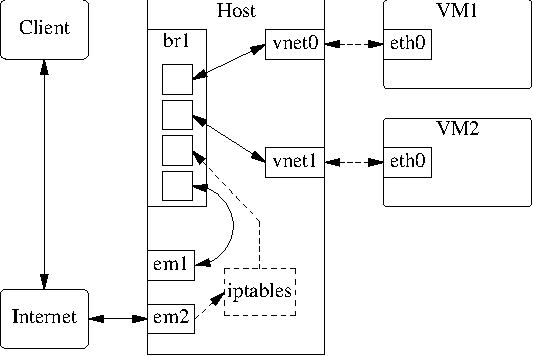
\includegraphics{graph/kvm_network.pdf}
\end{figure}


\section{qperf命令的使用}
\label{sec:qperfCmd}

我们在做网络服务器的时候,通常会很关心网络的带宽和延迟。因为我们的很多
协议都是request-response协议,延迟决定了最大的QPS,而带宽决定了最大的负
荷。 通常我们知道自己的网卡是什么型号,交换机什么型号,主机之间的物理距
离是多少,理论上是知道带宽和延迟是多少的。但是现实的情况是,真正的带宽
和延迟情况会有很多变数的,比如说网卡驱动,交换机跳数,丢包率,协议栈配
置,就实际速度而言,都很大的影响了数值的估算。 所以我们需要找到工具来实
际测量下。

SUSE11sp2发行版里面自带,方便安装,专业有效,能够针对TCP和RDMA进行带宽
和延迟的详细测试。

\begin{verbatim}
# zypper install -y qperf
\end{verbatim}

由于我们需要测试Infiniband的传输速率,在安装之前请先确认安装
了InfiniBand的相关包,比如librdmacm,libibverbs等。另外,也可以选择使用
源码包编译和安装qperf,但是需要注意,在安装之前也需要将infiniband相关的
包先安装上,否则RDMA的相关测试也将无法进行。

\begin{verbatim}
# zypper install -y librdmacm libibverbs
\end{verbatim}

\subsection{参数说明及示例}

qperf分为服务器端和客户端。客户端通过发送请求并获得响应来获得服务器端和
客户端之间的网络带宽以及延迟等信息。

\begin{tabular}{lp{20em}}
  \toprule
  参数名       & 参数说明 \\
  \midrule
  <server\_ip>	& 指定服务器的地址 \\
  time            & 指定网络测试时间。默认单位为秒,单位可以通过后缀为m,h,d指定为分钟,小时,天 \\
  conf	        & 测试输出中显示本地和远端服务器和操作系统配置 \\
  use\_bits\_per\_sec & 使用b(bit)而不是B(byte)来显示网络速度 \\
  precision 2	& 设置显示小数点后几位。这里设置为显示小数点后两位 \\
  verbose\_more	& 显示更详细的配置和状态信息 \\
  loop msg\_size:1:1025k:*2 	& loop表示对指定的指标值进行轮询。这里设置为对msg\_size轮询1,2,4,8…1024k,获得对应的测试结果,下次测试的指标值是上次测试指标值的*2倍 \\
  tcp\_bw	& 对tcp的带宽进行测试 \\
  tcp\_lat	& 对tcp的延迟进行测试 \\
  udp\_bw	& 对udp的带宽进行测试 \\
  udp\_lat	& 对udp的延迟进行测试 \\
  sdp\_bw	& 对sdp的延迟进行测试 \\
  sdp\_lat	& 对sdp的延迟进行测试 \\
\bottomrule
\end{tabular}

\section{iperf命令的使用}
\label{sec:iperfCmd}

iperf工具我们主要

首先到官网获取iperf工具,并把该工具放到合适的位置。
\begin{verbatim}
# wget https://iperf.fr/download/iperf_2.0.2/iperf_2.0.2-4_amd64
# chmod +x iperf_2.0.2-4_amd64
# mv iperf_2.0.2-4_amd64 /usr/bin/iperf
\end{verbatim}

\subsection{参数说明及示例}

\begin{tabular}{lp{25em}}
  \toprule
  参数名       & 参数说明 \\
  \midrule
  --server	& 以服务端模式运行 \\
  --udp	        & 指定测试UDP,默认为TCP带宽测试 \\
  --client <host>	& 以客户端模式运行,并连接<host> \\
  --bandwidth	& 指定测试中所使用的带宽,单位为[KM],默认为1Mbit/sec \\
  --time	        & 指定测试时间,单位为秒 \\
  --interval	& 指定多少时间间隔来报告测试结果,时间单位为秒 \\
  --format [kmKM]	& 指定报告的输出格式,单位分别为Kbits,Mbits,Kbytes,Mbytes \\
\bottomrule
\end{tabular}

\begin{enumerate}[itemsep=0pt,parsep=0pt]
\item 以太网UDP丢包率测试

\begin{verbatim}
A0304010:~ # iperf --server --udp 
A0305010:~ # iperf --udp --client 172.16.25.39 --interval 1 \
             --time 120 --bandwidth 900M
\end{verbatim}

\item InfiniBand网络UDP丢包率测试

\begin{verbatim}
# iperf --server --udp 
# iperf --udp --client 11.11.11.39 --interval 1 \
             --time 120 --bandwidth 1024M
\end{verbatim}

\item 如果不指定--udp选项,默认就是测试TCP带宽

\begin{verbatim}
A0304010:~ # iperf --server 
A0305010:~ # iperf --client 172.16.25.39  -f M
\end{verbatim}
\end{enumerate}

\section{vmstat命令的使用}
\label{sec:vmstatCmd}

Linux下vmstat输出释疑:

\begin{verbatim}
Vmstat
procs -----------memory---------- ---swap-- -----io---- --system-- ----cpu----
r b   swpd free buff cache          si so      bi bo      in cs    us sy id wa
0 0   100152 2436 97200 289740       0 1       34 45       99 33    0 0 99 0
\end{verbatim}

\begin{quote}
procs
r 列表示运行和等待cpu时间片的进程数,如果长期大于cpu个数,说明cpu不足,需要增加cpu。

b 列表示在等待资源的进程数,比如正在等待I/O、或者内存交换等。

memory
swpd 切换到内存交换区的内存数量(k表示)。如果swpd的值不为0,或者比较大,比如超过了100m,
     只要si、so的值长期为0,系统性能还是正常

free 当前的空闲页面列表中内存数量(k表示)

buff 作为buffer cache的内存数量,一般对块设备的读写才需要缓冲。

cache: 作为page cache的内存数量,一般作为文件系统的cache,如果cache较大,说明用到cache的
       文件较多,如果此时IO中bi比较小,说明文件系统效率比较好。

swap
si 由内存进入内存交换区数量。

so 由内存交换区进入内存数量。


IO
bi 从块设备读入数据的总量(读磁盘)(每秒kb)。

bo 块设备写入数据的总量(写磁盘)(每秒kb)


system 显示采集间隔内发生的中断数

in 列表示在某一时间间隔中观测到的每秒设备中断数。

cs 列表示每秒产生的上下文切换次数,如当cs比磁盘I/O和网络信息包速率高得多,都应进行进一步调查。



cpu 表示cpu的使用状态

us 列显示了用户方式下所花费 CPU 时间的百分比。us的值比较高时,说明用户进程消耗的cpu时间多,
   但是如果长期大于50\%,需要考虑优化用户的程序。

sy 列显示了内核进程所花费的cpu时间的百分比。这里us + sy的参考值为80\%,如果us+sy 大于
   80\%说明可能存在CPU不足。

wa 列显示了IO等待所占用的CPU时间的百分比。这里wa的参考值为30\%,如果wa超过30\%,说明IO等待严重,
   这可能是磁盘大量随机访问造成的,也可能磁盘或者磁盘访问控制器的带宽瓶颈造成的(主要是块操作)。

id 列显示了cpu处在空闲状态的时间百分比
\end{quote}


\section{iostat命令的使用}
\label{sec:iostatCmd}

\section{sar命令的使用}
\label{sec:sarCmd}

sar 命令行的常用格式:
\begin{verbatim}
sar [options] [-A] [-o file] t [n]
\end{verbatim}

在命令行中,n 和t 两个参数组合起来定义采样间隔和次数,t为采样间隔,是必
须有的参数,n为采样次数,是可选的,默认值是1,-o file表示将命令结果以二
进制格式存放在文件中,file 在此处不是关键字,是文件名。options 为命令行
选项,sar命令的选项很多,下面只列出常用选项:

\begin{table}[!htbp]
  \centering
  \begin{tabular}{ll}
    \toprule
    选项     & 说明 \\
    \midrule
    -A  & 所有报告的总和 \\
    -u  & CPU利用率 \\
    -v  & 进程、I节点、文件和锁表状态 \\
    -d  & 硬盘使用报告 \\
    -r  & 没有使用的内存页面和硬盘块 \\
    -g  & 串口I/O的情况(centos 5 中无此选项) \\
    -b  & 缓冲区使用情况 \\
    -a  & 文件读写情况 \\
    -c  & 系统调用情况 \\
    -R  & 进程的活动情况 \\
    -y  & 终端设备活动情况 \\
    -w  & 系统交换活动 \\
    \bottomrule
  \end{tabular}
  \caption{sar常用选项}
  \label{tab:sarOptions}
\end{table}

例一:使用命令行 sar -u t n

例如,每60秒采样一次,连续采样5次,观察CPU 的使用情况,并将采样结果以二
进制形式存入当前目录下的文件lavenliu中,需键入如下命令:

\begin{verbatim}
# sar -u -o lavenliu 60 5
SCO_SV   scosysv 3.2v5.0.5 i80386   10/01/2001
14:43:50   %usr   %sys  %wio    %idle(-u)
14:44:50   0     1    4      94
14:45:50   0     2    4      93
14:46:50   0     2    2      96
14:47:50   0     2    5      93
14:48:50   0     2    2      96
Average    0     2    4      94
\end{verbatim}

在显示内容包括:

\begin{verbatim}
%usr:CPU处在用户模式下的时间百分比。
%sys:CPU处在系统模式下的时间百分比。
%wio:CPU等待输入输出完成时间的百分比。
%idle:CPU空闲时间百分比。
\end{verbatim}

在所有的显示中,我们应主要注意\%wio和\%idle,\%wio的值过高,表示硬盘存
在I/O瓶颈,\%idle值高,表示CPU较空闲,如果\%idle值高但系统响应慢时,有
可能是CPU等待分配内存,此时应加大内存容量。\%idle值如果持续低于10,那么
系统的CPU处理能力相对较低,表明系统中最需要解决的资源是CPU。

如果要查看二进制文件lavenliu中的内容,则需键入如下sar命令:

\begin{verbatim}
# sar -u -f lavenliu
\end{verbatim}

可见,sar命令即可以实时采样,又可以对以往的采样结果进行查询。

例二:使用命行sar -v t n

例如,每30秒采样一次,连续采样5次,观察核心表的状态,需键入如下命令:

\begin{verbatim}
# sar -v 30 5
SCO_SV scosysv 3.2v5.0.5 i80386 10/01/2001
10:33:23 proc-sz ov inod-sz ov file-sz ov lock-sz   (-v)
10:33:53  305/ 321  0 1337/2764  0 1561/1706 0 40/ 128
10:34:23  308/ 321  0 1340/2764  0 1587/1706 0 37/ 128
10:34:53 305/ 321  0 1332/2764  0 1565/1706 0 36/ 128
10:35:23 308/ 321  0 1338/2764  0 1592/1706 0 37/ 128
10:35:53 308/ 321  0 1335/2764  0 1591/1706 0 37/ 128
\end{verbatim}

显示内容包括:

\begin{quote}
proc-sz:目前核心中正在使用或分配的进程表的表项数,由核心参数MAX-PROC控制。
inod-sz:目前核心中正在使用或分配的i节点表的表项数,由核心参数MAX-INODE控制
file-sz:目前核心中正在使用或分配的文件表的表项数,由核心参数MAX-FILE控制。
ov:     溢出出现的次数。
Lock-sz:目前核心中正在使用或分配的记录加锁的表项数,由核心参数MAX-FLCKRE控制。
\end{quote}

显示格式为: 实际使用表项/可以使用的表项数

显示内容表示,核心使用完全正常,三个表没有出现溢出现象,核心参数不需调
整,如果出现溢出时,要调整相应的核心参数,将对应的表项数加大。

例三:使用命行sar -d t n

例如,每30秒采样一次,连续采样5次,报告设备使用情况,需键入如下命令:
\begin{verbatim}
# sar -d 30 5
SCO_SV scosysv 3.2v5.0.5 i80386 10/01/2001
11:06:43 device %busy   avque   r+w/s  blks/s  avwait avserv (-d)
11:07:13 wd-0   1.47   2.75   4.67   14.73   5.50 3.14
11:07:43 wd-0   0.43   18.77   3.07   8.66   25.11 1.41
11:08:13 wd-0   0.77   2.78   2.77   7.26   4.94 2.77
11:08:43 wd-0   1.10   11.18   4.10   11.26   27.32 2.68
11:09:13 wd-0   1.97   21.78   5.86   34.06   69.66 3.35
Average wd-0   1.15   12.11   4.09   15.19   31.12 2.80
\end{verbatim}

显示内容包括:
\begin{verbatim}
device: sar命令正在监视的块设备的名字。
%busy: 设备忙时,传送请求所占时间的百分比。
avque: 队列站满时,未完成请求数量的平均值。
r+w/s: 每秒传送到设备或从设备传出的数据量。
blks/s: 每秒传送的块数,每块512字节。
avwait: 队列占满时传送请求等待队列空闲的平均时间。
avserv: 完成传送请求所需平均时间(毫秒)。
\end{verbatim}

在显示的内容中,wd-0是硬盘的名字,\%busy的值比较小,说明用于处理传送请求
的有效时间太少,文件系统效率不高,一般来讲,\%busy值高些,avque值低些,
文件系统的效率比较高,如果\%busy和avque值相对比较高,说明硬盘传输速度太
慢,需调整。

例四:使用命行sar -b t n

例如,每30秒采样一次,连续采样5次,报告缓冲区的使用情况,需键入如下命令:
\begin{verbatim}
# sar -b 30 5
SCO_SV scosysv 3.2v5.0.5 i80386 10/01/2001
14:54:59 bread/s lread/s %rcache bwrit/s lwrit/s %wcache pread/s pwrit/s (-b)
14:55:29 0  147  100  5  21  78   0   0
14:55:59 0  186  100  5  25  79   0   0
14:56:29 4  232   98  8  58  86   0   0
14:56:59 0  125  100  5  23  76   0   0
14:57:29 0   89  100  4  12  66   0   0
Average  1  156   99  5  28  80   0   0
\end{verbatim}

显示内容包括:
\begin{verbatim}
bread/s: 每秒从硬盘读入系统缓冲区buffer的物理块数。
lread/s: 平均每秒从系统buffer读出的逻辑块数。
%rcache: 在buffer cache中进行逻辑读的百分比。
bwrit/s: 平均每秒从系统buffer向磁盘所写的物理块数。
lwrit/s: 平均每秒写到系统buffer逻辑块数。
%wcache: 在buffer cache中进行逻辑读的百分比。
pread/s: 平均每秒请求物理读的次数。
pwrit/s: 平均每秒请求物理写的次数。
\end{verbatim}

在显示的内容中,最重要的是\%cache和\%wcache两列,它们的值体现着buffer的
使用效率,\%rcache的值小于90或者\%wcache的值低于65,应适当增加系
统buffer的数量,buffer数量由核心参数NBUF控制,使\%rcache达到90左
右,\%wcache达到80左右。但buffer参数值的多少影响I/O效率,增加buffer,应
在较大内存的情况下,否则系统效率反而得不到提高。

例五:使用命行sar -g t n
例如,每30秒采样一次,连续采样5次,报告串口I/O的操作情况,需键入如下命令:
\begin{verbatim}
# sar -g 30 5
SCO_SV scosysv 3.2v5.0.5 i80386  11/22/2001
17:07:03  ovsiohw/s  ovsiodma/s  ovclist/s (-g)
17:07:33   0.00   0.00   0.00
17:08:03   0.00   0.00   0.00
17:08:33   0.00   0.00   0.00
17:09:03   0.00   0.00   0.00
17:09:33   0.00   0.00   0.00
Average    0.00   0.00   0.00
\end{verbatim}

显示内容包括:
\begin{verbatim}
ovsiohw/s:每秒在串口I/O硬件出现的溢出。
ovsiodma/s:每秒在串口I/O的直接输入输出通道高速缓存出现的溢出。
ovclist/s :每秒字符队列出现的溢出。
\end{verbatim}

在显示的内容中,每一列的值都是零,表明在采样时间内,系统中没有发生串口
I/O溢出现象。

sar命令的用法很多,有时判断一个问题,需要几个sar命令结合起来使用,比如,
怀疑CPU存在瓶颈,可用sar -u 和sar -q来看,怀疑I/O存在瓶颈,可用sar -b、
sar -u和sar-d来看。

\section{ip命令的使用}
\label{sec:ipCmd}

\subsection{显示IP信息}

